% 图 84.6 —— 由 `checks/emit_hand.py` 自动拼出（probe 精测 + prims2 图元分解）
%%
% ⚠ 这是**稿子不是成品**：跑 `checks/checkhand.py 84.6` 看指标 + 看叠合图。
%%
%% ⚠ 待核：
%   · 本图 probe 报出阴影族 1 个 —— **本脚本不生成阴影**（要照原书手写）；prims2 的 strokes 里可能含阴影线，核对时留意别画重
%   · 可疑字形 1 项（空心圈 ⊙ 常被认成字母 o）—— 见文件末
%%
\documentclass[12pt]{standalone}
\usepackage{fontspec}
\setsansfont{Arial}
\newfontfamily\mfallback{DejaVu Sans}
\usepackage{tikz}
\begin{document}
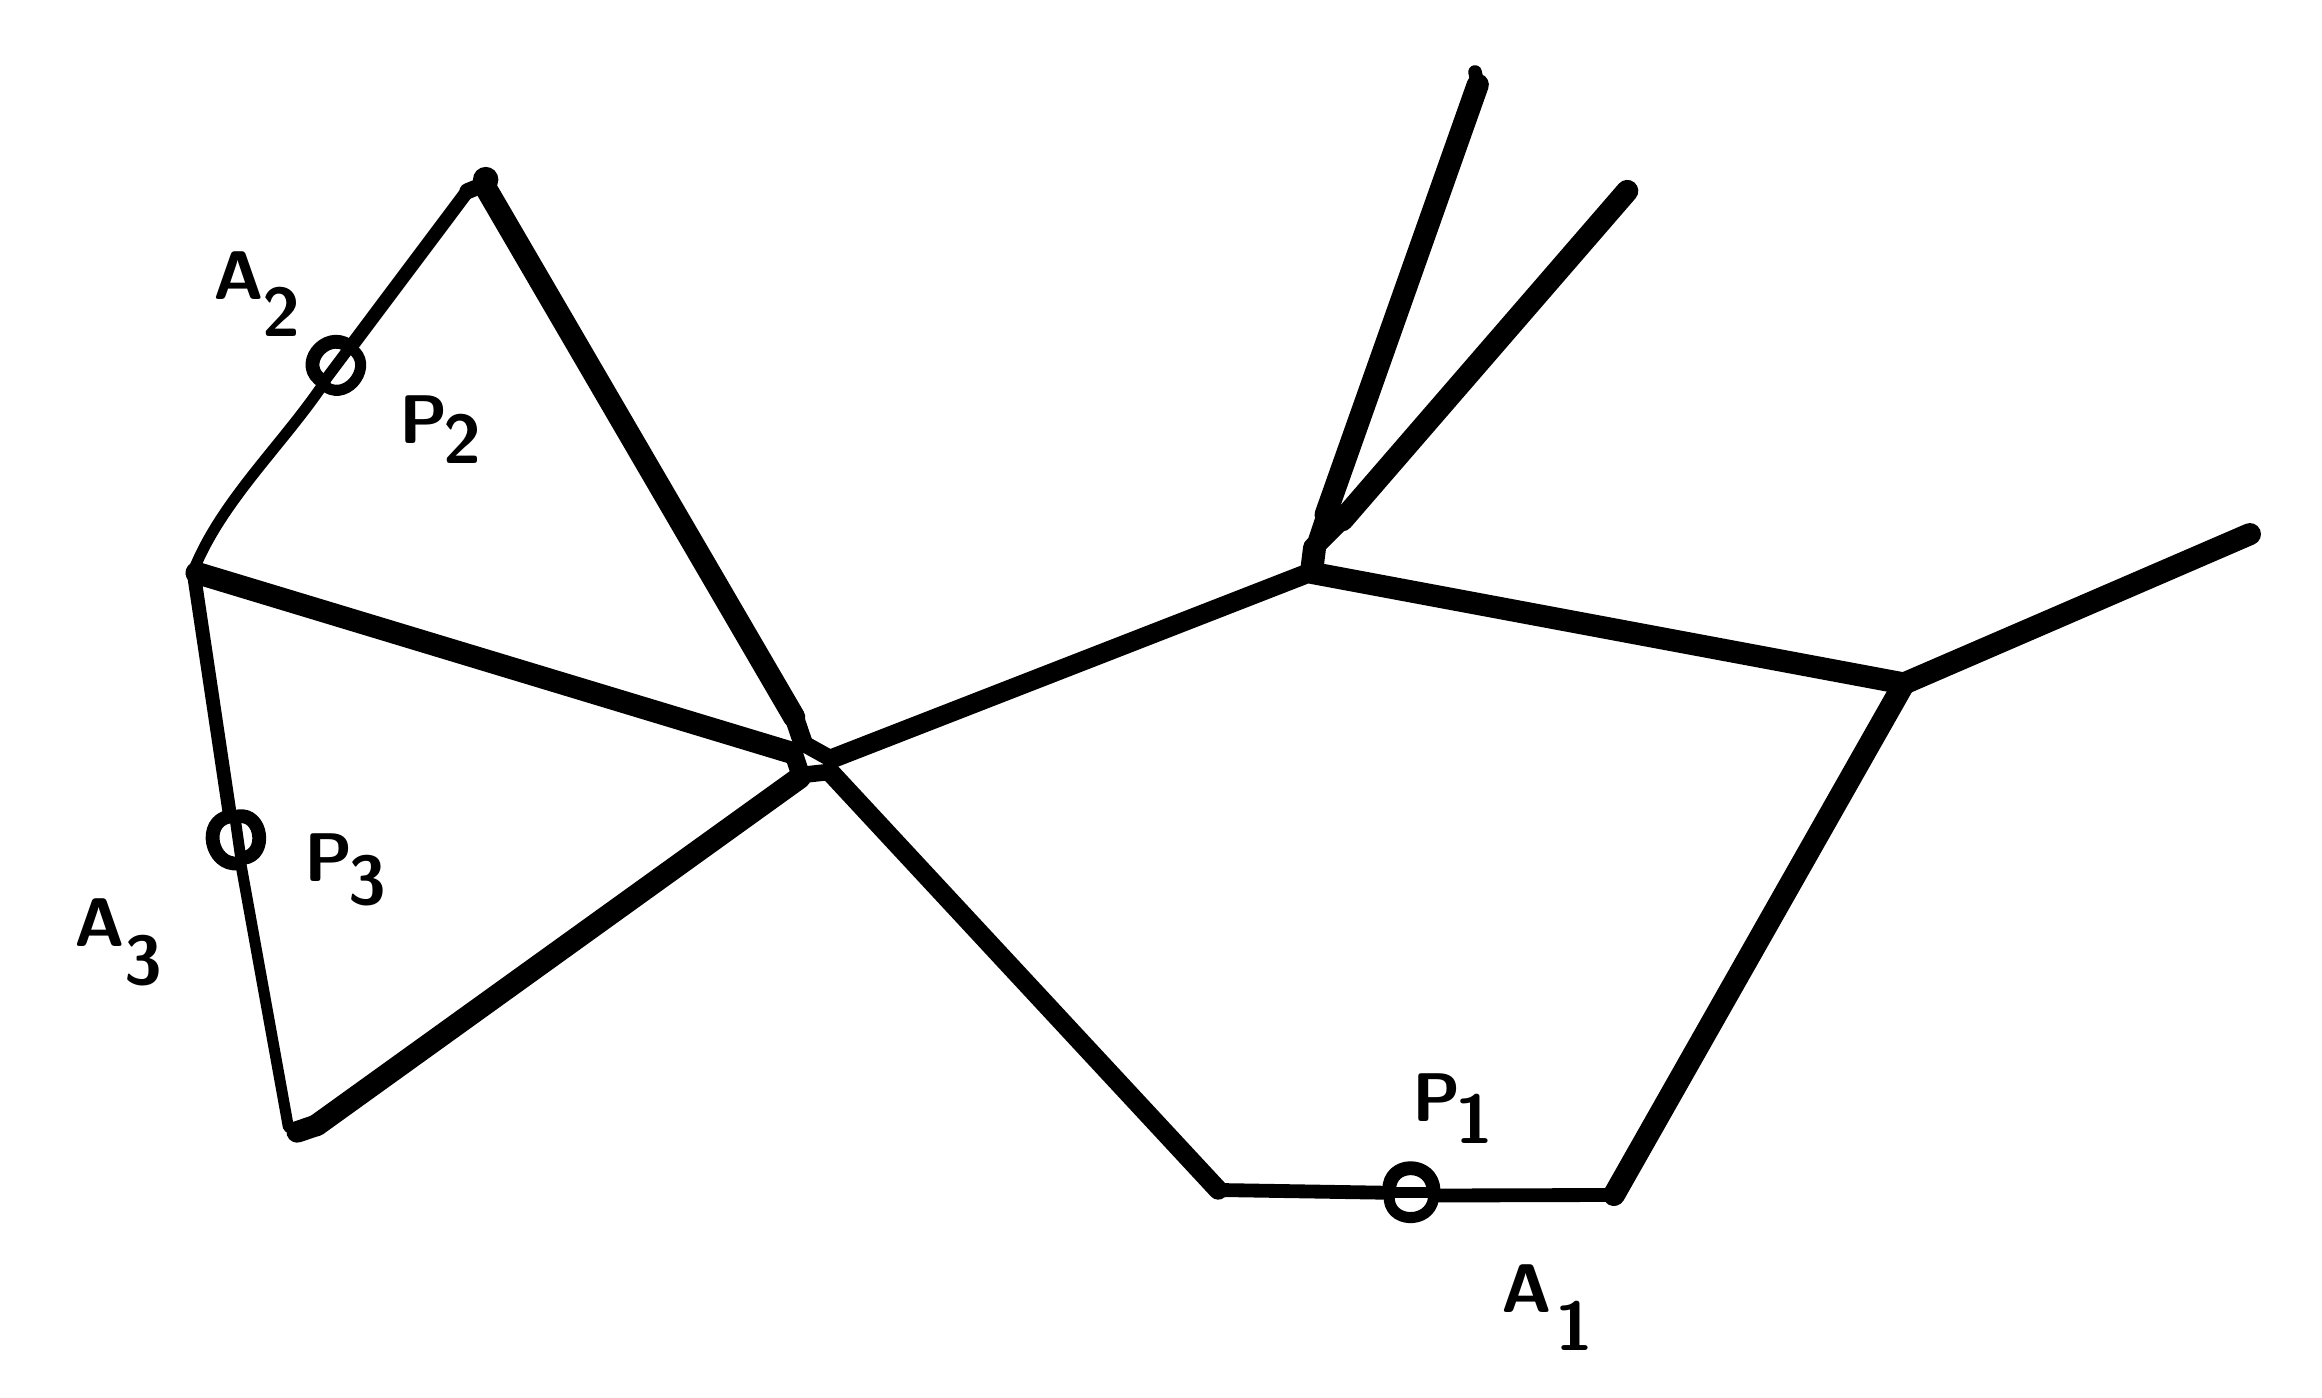
\begin{tikzpicture}[x=1pt, y=-1pt, line width=6.0pt, line cap=round, line join=round]

  %% ════ 填充区（prims2 的 fills）════

  %% ════ 直线段（prims2 的 strokes）════
  \draw[line width=6.0pt] (281.0,259.0) -- (290.0,264.0);
  \draw[line width=8.0pt] (464.0,197.0) -- (678.0,237.0);
  \draw[line width=4.0pt] (116.0,116.0) -- (107.0,128.0);
  \draw[line width=6.7pt] (279.0,269.0) -- (277.0,263.0);
  \draw[line width=5.8pt] (164.0,57.0) -- (158.9,59.1);
  \draw[line width=5.0pt] (158.9,59.1) -- (117.0,115.0);
  \draw[line width=8.0pt] (469.0,176.0) -- (524.0,20.6);
  \draw[line width=4.9pt] (524.0,20.6) -- (523.0,16.0);
  \draw[line width=6.5pt] (469.0,176.0) -- (465.0,188.0);
  \draw[line width=5.7pt] (469.0,176.0) -- (474.0,178.0);
  \draw[line width=8.0pt] (279.0,271.0) -- (104.4,396.6);
  \draw[line width=7.8pt] (104.4,396.6) -- (97.4,399.0);
  \draw[line width=3.8pt] (97.4,399.0) -- (94.2,397.2);
  \draw[line width=4.0pt] (94.2,397.2) -- (77.0,302.0);
  \draw[line width=8.0pt] (475.0,178.0) -- (578.0,59.0);
  \draw[line width=8.0pt] (61.0,197.0) -- (276.0,262.0);
  \draw[line width=6.5pt] (474.0,179.0) -- (465.0,188.0);
  \draw[line width=4.0pt] (75.0,286.0) -- (77.0,300.0);
  \draw[line width=5.0pt] (509.0,422.0) -- (573.2,421.8);
  \draw[line width=8.0pt] (573.2,421.8) -- (678.0,237.0);
  \draw[line width=7.0pt] (291.0,264.0) -- (463.0,197.0);
  \draw[line width=3.0pt] (290.0,265.0) -- (290.0,268.0);
  \draw[line width=6.0pt] (280.0,270.0) -- (289.0,269.0);
  \draw[line width=4.0pt] (507.0,421.0) -- (493.0,421.0);
  \draw[line width=8.0pt] (803.0,183.0) -- (678.0,237.0);
  \draw[line width=5.0pt] (60.0,197.0) -- (73.0,284.0);
  \draw[line width=7.0pt] (290.0,269.0) -- (430.2,420.0);
  \draw[line width=5.0pt] (430.2,420.0) -- (491.0,421.0);
  \draw[line width=8.3pt] (464.0,196.0) -- (465.0,188.0);
  \draw[line width=8.0pt] (165.0,57.0) -- (277.0,249.2);
  \draw[line width=7.0pt] (277.0,249.2) -- (280.0,258.0);

  %% ════ 曲线（prims2 的 curves —— 三段式，坐标同为 (y,x)）════
  \draw[line width=4.0pt] (106.0,130.0) .. controls (91.0,151.7) and (69.7,171.7) .. (60.0,196.0);
  \draw[line width=4.0pt] (508.0,423.0) .. controls (506.7,432.8) and (491.2,432.1) .. (492.0,422.0);
  \draw[line width=5.0pt] (73.0,285.0) .. controls (62.8,286.8) and (66.2,303.0) .. (76.0,302.0);
  \draw[line width=5.0pt] (76.0,285.0) .. controls (84.8,283.6) and (86.8,299.0) .. (78.0,300.0);
  \draw[line width=5.0pt] (508.0,420.0) .. controls (507.6,409.6) and (491.8,409.4) .. (492.0,420.0);
  \draw[line width=4.0pt] (108.0,130.0) .. controls (116.0,134.9) and (125.5,121.6) .. (117.0,116.0);
  \draw[line width=5.0pt] (107.0,128.0) .. controls (96.9,122.4) and (107.6,109.0) .. (116.0,115.0);

  %% ════ 实心点 ════
  \fill (165.5,54.9) circle (4.6);

  %% ════ 标签（probe 直接给的 \node 行）════
  %% ⚠ 全部补了 fill=white：文字在最上层，否则与曲线交叉干扰
     \node[anchor=center,inner sep=0pt,fill=white,font=\fontsize{29.6}{37.0}\selectfont] at (76.2,89.5) {\textsf{\textbf{\textit{A}}}};   % box(64,78,19,22)
     \node[anchor=center,inner sep=0pt,fill=white,font=\fontsize{24.7}{30.9}\selectfont] at (91.6,102.9) {\textsf{\textbf{2}}};   % box(85,94,12,17)
     \node[anchor=center,inner sep=0pt,fill=white,font=\fontsize{29.8}{37.3}\selectfont] at (143.0,141.5) {\textsf{\textbf{\textit{P}}}};   % box(132,129,18,23)
     \node[anchor=center,inner sep=0pt,fill=white,font=\fontsize{23.6}{29.6}\selectfont] at (157.1,148.9) {\textsf{\textbf{2}}};   % box(151,140,11,17)
     \node[anchor=center,inner sep=0pt,fill=white,font=\fontsize{29.2}{36.4}\selectfont] at (108.9,300.0) {\textsf{\textbf{\textit{P}}}};   % box(98,288,18,22)
     \node[anchor=center,inner sep=0pt,fill=white,font=\fontsize{23.0}{28.7}\selectfont] at (122.9,308.1) {\textsf{\textbf{3}}};   % box(117,299,11,17)
     \node[anchor=center,inner sep=0pt,fill=white,font=\fontsize{29.6}{37.0}\selectfont] at (26.2,323.5) {\textsf{\textbf{\textit{A}}}};   % box(14,312,19,22)
     \node[anchor=center,inner sep=0pt,fill=white,font=\fontsize{23.0}{28.7}\selectfont] at (41.9,337.1) {\textsf{\textbf{3}}};   % box(36,328,11,17)
     \node[anchor=center,inner sep=0pt,fill=white,font=\fontsize{29.8}{37.3}\selectfont] at (509.0,386.5) {\textsf{\textbf{\textit{P}}}};   % box(498,374,18,23)
     \node[anchor=center,inner sep=0pt,fill=white,font=\fontsize{23.7}{29.7}\selectfont] at (522.8,394.4) {\textsf{\textbf{1}}};   % box(516,386,8,16)
     \node[anchor=center,inner sep=0pt,fill=white,font=\fontsize{30.3}{37.9}\selectfont] at (541.8,455.5) {\textsf{\textbf{\textit{A}}}};   % box(529,444,20,22)
     \node[anchor=center,inner sep=0pt,fill=white,font=\fontsize{23.7}{29.7}\selectfont] at (558.8,469.4) {\textsf{\textbf{1}}};   % box(552,461,8,16)

  % 钉死画布：否则超出的图元/控制点会把页面撑大，1:1 回比就失准
  \pgfresetboundingbox
  \path[use as bounding box] (0,0) rectangle (819,485);
\end{tikzpicture}
\end{document}

% ⚠ 待核清单（probe 拿不准，人眼过一遍）：
%   · 未识别/跳过：⑤ 跳过/未识别的字形
